\section{Node Collapse}

\revise{Given the new model to represent a node, two nodes $v_i^j$, $v_i^k$ with the same code segments (i.e., $cs_i^j = cs_i^k$ and $c_i^j = c_i^k$) are collapsed into one node $v_i^h$, where $v_i^h = <cs_i^j, c_i^j, \max{\eta_i^j, \eta_i^k}+1>$.  To ensure dependencies of the DAG are not violated, we replace the edges that start from $v_i^j$ and $v_i^k$  to start from $v_i^h$, i.e., the child nodes of $v_i^h$ are given as a union of the child nodes of $v_i^j$ and $v_i^k$, $child(v_i^h) = child(v_i^j) \cup child(v_i^k)$. Similarly, parent nodes of $v_i^h$ are given as a union of the parent nodes of $v_i^j$ and $v_i^k$, i.e., $parent(v_i^h) = parent(v_i^j) \cup parent(v_i^k)$.}

\begin{figure}
  \centering
  \begin{subfigure}[b]{0.4\textwidth}{
      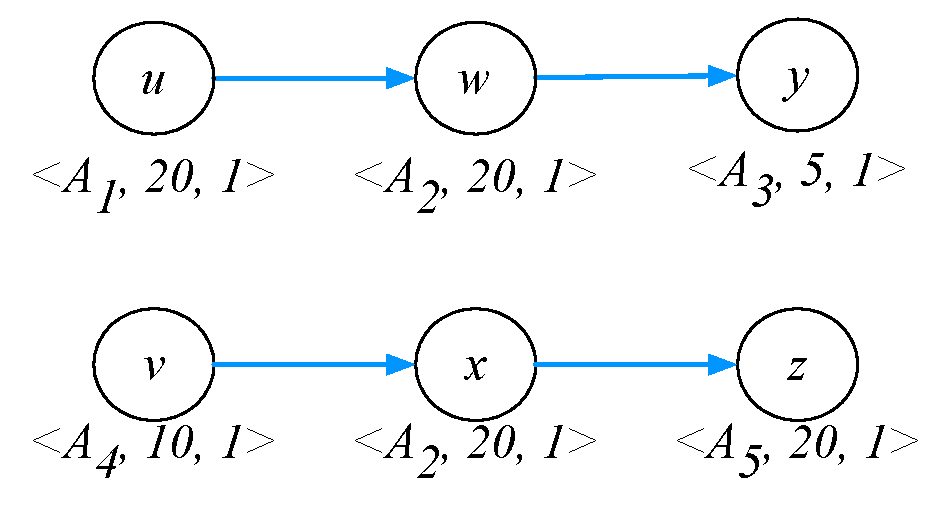
\includegraphics[width=\textwidth]{beforeCollapse}
      \caption{Before Collapse}
      \label{fig:before-collapse}
    }
  \end{subfigure} \quad
  \begin{subfigure}[b]{0.4\textwidth}{
      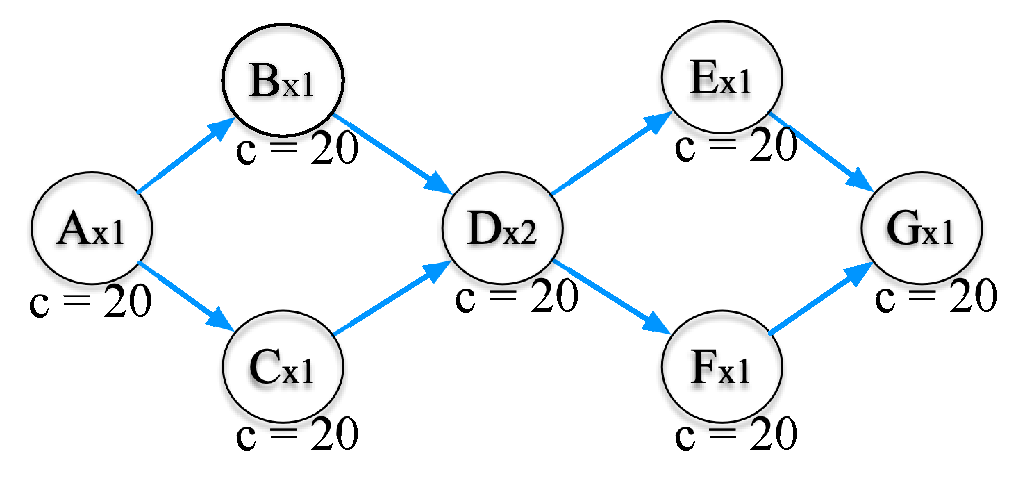
\includegraphics[width=\textwidth]{afterCollapse}
      \caption{After Collapse}
      \label{fig:after-collapse}
    }
  \end{subfigure}
  \caption{DAG Node Change from Thread to Code Segment}
  \label{fig:dag-collapse}
\end{figure}



Figure~\ref{fig:dag-collapse} illustrates the proposed change. Nodes in
Figure~\ref{fig:before-collapse} are labeled with the code segment
they are associated with. Two nodes of ${B}$ are collapsed in
Figure~\ref{fig:after-collapse}, where each node is attributed with
the number of threads executed over the code segment.


\section{Candidacy for collapse}

\subsection{Conditions for Candidacy of Collapse}
For a task ${\task{i} \in \tasks{}}$, associated DAG ${\Dag{i}
  \in \dagset{}}$, where ${\Dag{i} = (V, E)}$,
the nodes ${u,v \in V}$ qualify as \emph{candidates} for collapse if
and only if the following conditions are true:
\begin{enumerate}
  \item Nodes ${u}$ and ${v}$ refer to execution of the same object.
  \item Collapsing ${u}$ and ${v}$ cannot not introduce a cycle in ${G_i}$.
  \item The sum of the individual worst-case execution times of ${u}$
    and ${v}$ is greater than the collapsed worst-case execution time
    of ${u}$ and ${v}$ i.e. ${c(u) + c(v) > c(u + v)}$.
\end{enumerate}

\revise{Following paragraph should state: One property of collapse is
  that loops cannot be introduced for two nodes to remain candidates
  of collapse.
}
In a DAG ${G_i = (V_i, E_i)}$, collapsing two nodes that represent the
execution of the same code segment may result in a violation of the
DAG. For example, Fig~\ref{fig:dag-violation} shows one such example
where collapsing two nodes with the same code segment $B$ results in a
loop inside the DAG. In this section, we derive the necessary and
sufficient condition for a pair of nodes when satisfied does not
result in a DAG violation after a collapse.

\revise{Needed: introductory paragraph to state the following theorem
  provides a condition for ensuring collapse does not introduce loops}

\begin{figure}
  \centering
  \begin{subfigure}[b]{0.48\textwidth}{
      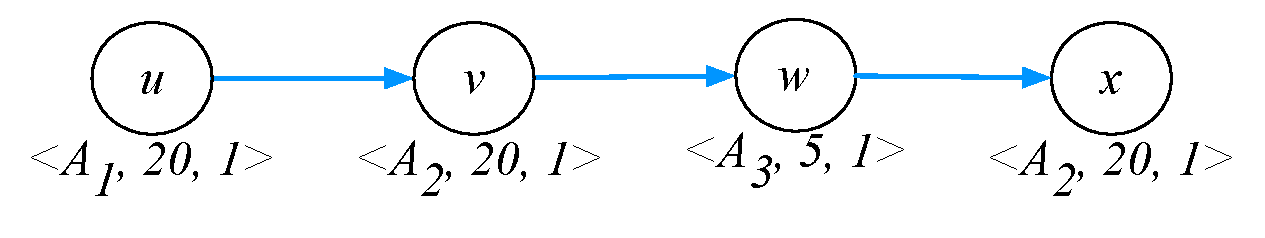
\includegraphics[width=\textwidth]{beforeViolation}
      \caption{Before Collapse}
      \label{fig:beforeViolation}
    }
  \end{subfigure}~
  \begin{subfigure}[b]{0.33\textwidth}{
      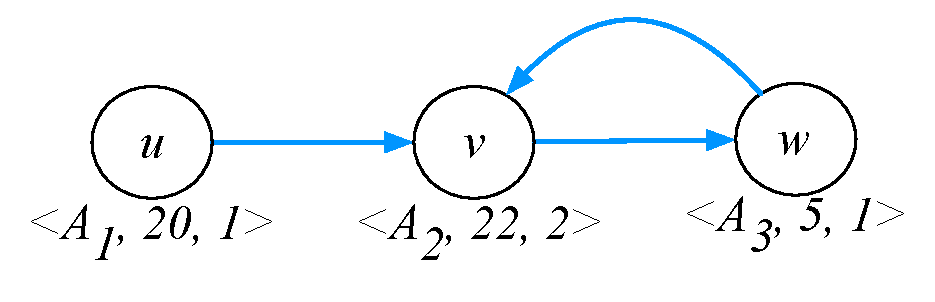
\includegraphics[width=\textwidth]{afterViolation}
      \caption{After Collapse}
      \label{fig:afterViolation}
    }
  \end{subfigure}
  \caption{Collapse of two nodes can result in a loop inside the DAG task}
  \label{fig:dag-violation}
\end{figure}

\revise{expand both definitions} \\
\textbf{Definition ${u \prec v}$} -- indicates that ${u}$ appears
before ${v}$ in a topological sort of ${G}$. \\
\textbf{Definition ${d(u, v)}$} -- is the greatest number of edges
along a directed path from ${u}$ to ${v}$ in ${G}$. When no path
exists, ${d(u,v) = 0}$.

\begin{theorem}[Candidacy for Collapse]
  For a DAG ${G = (V, E)}$ and nodes ${u, v \in V}$ where ${u \prec
    v}$, ${u}$ and ${v}$ can be collapsed without introducing a loop
  if and  only if ${d(u, v) \le 1}$.
\end{theorem}


\begin{theorem}[Candidacy for collapse] \label{thrm:candidacy-collapse} Two nodes $v_i^j$ and $v_i^k$ in a DAG task $\tau_i$ when collapsed do not introduce a loop if and only if $d(v_i^j, v_i^k) \le 1$ and $d(v_i^k, v_i^j) \le 1$, where $d(v_i^j, v_i^k)$ is the length of the longest path between $v_i^j$ and $v_i^k$ as obtained by depth first search. \end{theorem}
\begin{proof}
%The proof is divided into two parts
We divide the proof into two parts. We first prove that the condition $d(v_i^j, v_i^k) \le 1$ and $d(v_i^k, v_i^j) \le 1$ is a necessary condition for candidacy and latter we prove that the condition is a sufficient condition.

%First part - necessary part - to prove that if the constraint is violated then it will result a violation of the dag 
If the condition is not satisfied $d(v_i^j, v_i^k) \le 1$ and $d(v_i^k, v_i^j) \le 1$, then it implies that there is a path from $v_i^j$ to $v_i^k$ or a path from $v_i^k$ and $v_i^j$ with length greater than 1, i.e., $\exists p1 \  such \  that p1 = {v_i^j, v_i^l, \cdots , v_i^k} or p1 = {v_i^k, v_i^l, \cdots , v_i^l}$. When nodes $v_i^j$ and $v_i^k$ are collapsed into $v_i^h$, $p1$ will be modified to ${v_i^h, v_i^l, \cdots , v_i^h}$ which forms a loop. 

%Second part -  sufficient part - if the constraint is met there is no other source of a loop
To prove the sufficient condition, we first prove the contra-positive to be true, i.e., a DAG violation occurs only when the condition $d(v_i^j, v_i^k) \le 1$ and $d(v_i^k, v_i^j) \le 1$ is true. A DAG violation in the collapsed DAG implies that there exists a path $p1$ in the collapsed DAG given by $v_i^h, v_i^l, \cdots , v_i^h$ with a length greater than or equal to 2.  Since there are no loops in the original DAG, only a collapsed node can cause a loop in the collapsed DAG. Therefore, $v_i^h$ should be the collapsed node. In the original DAG, one node of $v_i^h$ corresponds to $v_i^j$ and the other node corresponds to $v_i^k$. In the original DAG, $p1$ must correspond to ${v_i^j, v_i^l, \cdots , v_i^k} or {v_i^k, v_i^l, \cdots , v_i^l}$. Thus, a DAG violation in the collapsed DAG implies that there exists a path from $v_i^j$ to $v_i^k$  or $v_i^k$ and $v_i^j$ with a length greater than or equal to 2. 

Therefore, we can conclude that two nodes $v_i^j$ and $v_i^k$ in a DAG task $\tau_i$ when collapsed do not introduce a loop if and only if $d(v_i^j, v_i^k) \le 1$ and $d(v_i^k, v_i^j) \le 1$.
\end{proof}

In summary, we define two nodes $v_i^j$ and $v_i^k$ to be {\textbf candidates for collapse} if they have the same code block and $d(v_i^j, v_i^k) \le 1$ and $d(v_i^k, v_i^j) \le 1$, where $d(v_i^j, v_i^k)$ is the length of the longest path between $v_i^j$ and $v_i^k$.
